\documentclass{beamer}

\usepackage{tikz}
\usepackage{pdfpages}
\usetikzlibrary{shapes,snakes}

\newcommand{\smtc}[1]{\texttt{#1}}
\newcommand{\smtcuc}[1]{\texttt{\color{blue}#1}}
\newcommand{\tdots}{$...$}

% switch off the fancy navigation symbols
\setbeamertemplate{navigation symbols}{}

\title[SMT-COMP 2018]{${}$\\[3.5em]13th International\\
Satisfiability Modulo Theories\\
Competition\\[.7em]
SMT-COMP 2018\\[3em]}

\author{Matthias Heizmann \and Aina Niemetz\\ \and Giles Reger \and
  \underline{Tjark Weber}}

\institute{}

\date{}

\logo{\vspace{2.7cm}\includegraphics[width=\textwidth]{laurels}\hspace{.8cm}}

\begin{document}

%%%%%%%%%%%%%%%%%%%%%%%%%%%%%%%%%%%%%%%%%%%%%%%%%%%%%%%%%%%%%%%%%%%%%%%%%%%%%%%%

\frame{\titlepage}
\logo{}

%%%%%%%%%%%%%%%%%%%%%%%%%%%%%%%%%%%%%%%%%%%%%%%%%%%%%%%%%%%%%%%%%%%%%%%%%%%%%%%%

\section{}% leave this empty
\subsection{}% leave this empty

%%%%%%%%%%%%%%%%%%%%%%%%%%%%%%%%%%%%%%%%%%%%%%%%%%%%%%%%%%%%%%%%%%%%%%%%%%%%%%%%

\begin{frame}{Outline}
  \begin{itemize}
  \item Design and scope

    \smallskip

    \begin{itemize}
    \item Main changes from last year's competition
    \end{itemize}

    \vfill

  \item Short presentation of solvers

    \smallskip

    \begin{itemize}
    \item TODO: Solver names in alphabetical order
    \end{itemize}

    \vfill

  \item Selected results
  \end{itemize}
\end{frame}

%%%%%%%%%%%%%%%%%%%%%%%%%%%%%%%%%%%%%%%%%%%%%%%%%%%%%%%%%%%%%%%%%%%%%%%%%%%%%%%%

\begin{frame}{}
  \begin{center}
    \vfill
      {\huge \structure{Design and Scope}}
    \vfill
  \end{center}
\end{frame}

%%%%%%%%%%%%%%%%%%%%%%%%%%%%%%%%%%%%%%%%%%%%%%%%%%%%%%%%%%%%%%%%%%%%%%%%%%%%%%%%

\begin{frame}{Background}
  SMT-COMP is an annual competition between SMT solvers.
  \vfill
  It was first held in 2005
  \medskip
  \begin{itemize}
  \item to spur adoption of the common, community-designed SMT-LIB
    format, and
    \smallskip
  \item to spark further advances in SMT by stimulating improvement
    in solver implementations.
  \end{itemize}
  \vfill
  It has evolved into the world's largest$^*$ ATP competition.
\end{frame}

%%%%%%%%%%%%%%%%%%%%%%%%%%%%%%%%%%%%%%%%%%%%%%%%%%%%%%%%%%%%%%%%%%%%%%%%%%%%%%%%

\begin{frame}{SMT-COMP -- Procedure}

  \medskip

  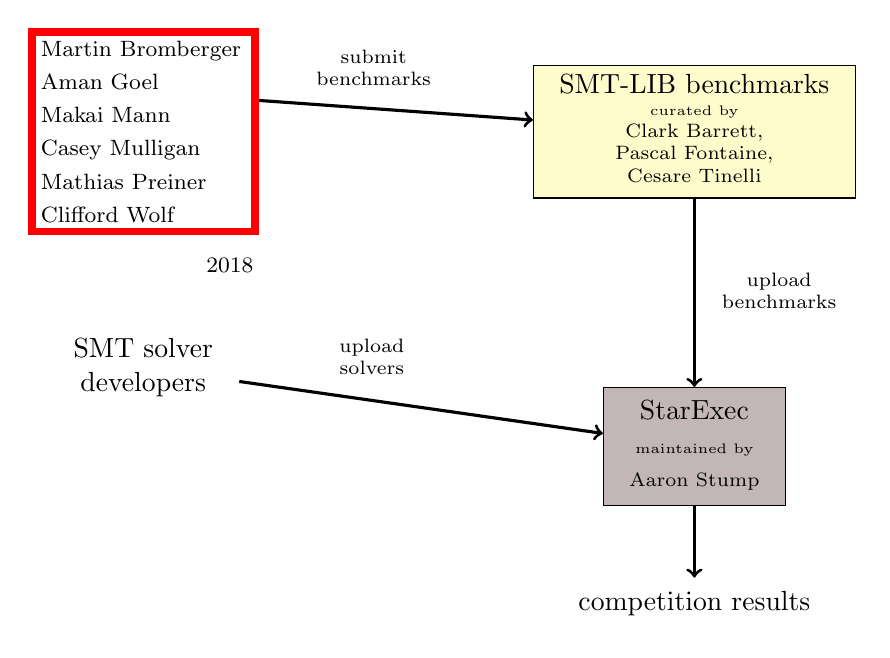
\begin{tikzpicture}
    \node (SMTusers) [] at (-7,5.5) {\begin{tabular}{c}SMT-LIB\\ users\end{tabular}};
    \node (SMTbenchmarks) [draw, rectangle, fill=yellow!20] at (0,5) {\scriptsize\begin{tabular}{c}
      \normalsize SMT-LIB benchmarks\\ \tiny curated by\\ Clark Barrett,\\ Pascal Fontaine,\\ Cesare Tinelli
    \end{tabular}};
    \node (SMTsolvers) [] at (-7,2) {\begin{tabular}{c}SMT solver\\ developers\end{tabular}};
    \node (starexec) [draw, rectangle, fill=lightgray!95!red] at (0,1) {\begin{tabular}{c}StarExec\\ \tiny maintained by\\ \scriptsize Aaron Stump\end{tabular}};
    \node (results) [] at (0,-1) {\begin{tabular}{c}competition results\end{tabular}};

    \draw[->,thick,line width=0.4mm] (SMTusers) to node[auto, pos=0.2] {\scriptsize \begin{tabular}{c}submit\\ benchmarks\end{tabular}} (SMTbenchmarks);
    \draw[->,thick,line width=0.4mm] (SMTsolvers) to node[auto, pos=0.2] {\scriptsize \begin{tabular}{c}upload\\ solvers\end{tabular}} (starexec);
    \draw[->,thick,line width=0.4mm] (SMTbenchmarks) to node[auto] {\scriptsize \begin{tabular}{c}upload\\ benchmarks\end{tabular}} (starexec);
    \draw[->,thick,line width=0.4mm] (starexec) to node[auto] {} (results);

    \pause

    \node [fill=white,draw=red,line width=1mm] at (-7,5) {
      \begin{minipage}{26mm}
        {\footnotesize
          Martin Bromberger\\
          Aman Goel\\
          Makai Mann\\
          Casey Mulligan\\
          Mathias Preiner\\
          Clifford Wolf
        }
      \end{minipage}
    };
    \node at (-5.9,3.3) {\footnotesize 2018};
  \end{tikzpicture}

\end{frame}

%%%%%%%%%%%%%%%%%%%%%%%%%%%%%%%%%%%%%%%%%%%%%%%%%%%%%%%%%%%%%%%%%%%%%%%%%%%%%%%%

\begin{frame}{Main Track}
  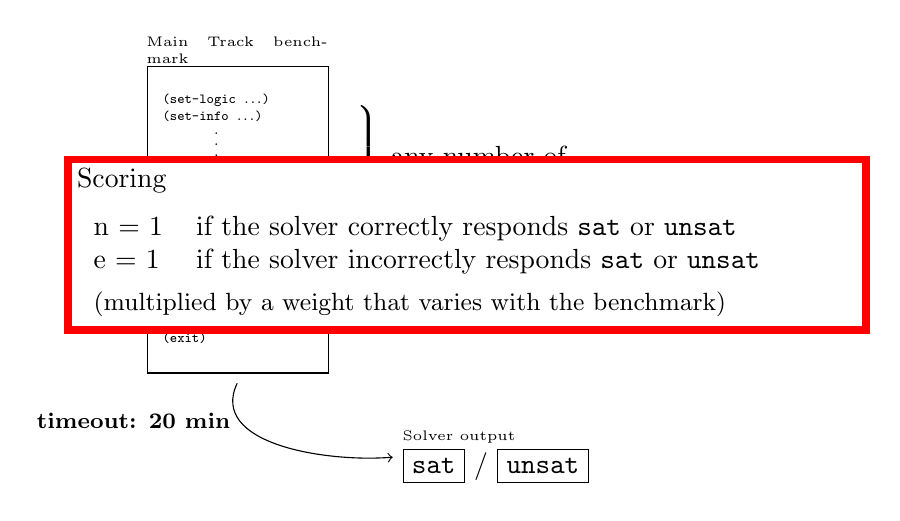
\begin{tikzpicture}
    \node (maintrackscript) at (-4.1,0) {
      \begin{minipage}{23mm}
        \tiny
        
        Main Track benchmark
        
        \fbox{
          \parbox{20mm}{
            \strut\\
            \smtc{(set-logic \tdots)}\\
            \smtc{(set-info \tdots)}\\[-1mm]
            $\phantom{mmm}\vdots$\\
            \smtc{(declare-sort \tdots)}\\
            \smtc{(define-sort \tdots)}\\
            \smtc{(declare-fun \tdots)}\\
            \smtc{(define-fun \tdots)}\\
            \smtc{(assert term0)}\\
            \smtc{(assert term1)}\\
            \smtc{(assert term2)}\\[-1mm]
            $\phantom{mmm}\vdots$\\
            \smtc{(check-sat)}\\
            \smtc{(exit)}\\
            \strut
        }}
      \end{minipage}
    };
    
    \node[anchor=west] at (-3.1,0) {
      $\left.\begin{array}{l}\\ \\ \\ \\ \\ \\\end{array}\right\}$
        \parbox{60mm}{any number of\\ {\footnotesize ${}$\quad \smtc{set-info}, \smtc{declare-sort}, \smtc{define-sort},\\ ${}$\quad \smtc{declare-fun}, \smtc{define-fun}, \smtc{assert}}\\
          commands}
    };
    
    \node[anchor=west] at (-2.7,-1.5) {$\leftarrow$ one \smtc{check-sat} command};
    
    \pause
    
    \node (solveroutput) at (0,-3.2) {
      \begin{minipage}{40mm}
        {\tiny Solver output}
        
        \fbox{\smtc{sat}} /
        \fbox{\smtc{unsat}}
      \end{minipage}
    };
    \draw[->, bend right, out=-90] (maintrackscript.south) to node[left,pos=0.25]{\footnotesize\textbf{timeout: 20 min}} (solveroutput.west);
    
    \pause
    
    \node[fill=white,draw=red, line width=1mm, anchor=west] (scoring) at (-6.3,-.5) {
      \begin{minipage}{99mm}
        Scoring
        
        \medskip
        
        \begin{tabular}{ll}
          n = 1 & if the solver correctly responds \smtc{sat} or \smtc{unsat}\\
          e = 1 & if the solver incorrectly responds \smtc{sat} or \smtc{unsat}\\[.3em]
          \multicolumn{2}{l}{\small (multiplied by a weight that varies with the benchmark)}
        \end{tabular}
      \end{minipage}
    };
  \end{tikzpicture}
\end{frame}

%%%%%%%%%%%%%%%%%%%%%%%%%%%%%%%%%%%%%%%%%%%%%%%%%%%%%%%%%%%%%%%%%%%%%%%%%%%%%%%%

\begin{frame}{Application Track}
  \begin{tikzpicture}
    \node (applicationtrackscript) at (-4.1,0) {
      \begin{minipage}{23mm}
        \tiny

        Application Track\\
        benchmark

        \fbox{
          \parbox{20mm}{
            \strut\\
            \smtc{(set-logic \tdots)}\\[-1mm]
            $\phantom{mmm}\vdots$\\
            \smtc{(check-sat)}\\[-1mm]
            $\phantom{mmm}\vdots$\\
            \smtc{(check-sat)}\\[-1mm]
            $\phantom{mmm}\vdots$\\
            \smtc{(check-sat)}\\[-1mm]
            $\phantom{mmm}\vdots$\\
            \smtc{(check-sat)}\\
            \smtc{(exit)}\\
            \strut
        }}
      \end{minipage}
    };

    \node at (0,3.2) {
      \begin{minipage}{\textwidth}
        \only<1>{Application track benchmarks may contain {\bf
            multiple} \texttt{check-sat} commands, as well as
          \texttt{push} and \texttt{pop} commands.}
        \only<2->{Application track benchmarks are fed to the solver
          {\bf incrementally} by a trace executor.}
      \end{minipage}
    };

    \only<1>{%
      \node[anchor=west] at (-3.3,-.2) {
        $\left.\begin{array}{l}\\ \\ \\ \\ \\ \\\end{array}\right\}$
          \parbox{61mm}{any number of\\ {\footnotesize ${}$\quad \smtc{set-info}, \smtc{declare-sort}, \smtc{define-sort},\\ ${}$\quad \smtc{declare-fun}, \smtc{define-fun}, \smtc{assert}, \smtc{push},\\ ${}$\quad \smtc{pop}, \smtc{check-sat}}\\
            commands}
      };
    }

    \pause
    
    \node (timeout) at (1.8,-3) {
      \begin{minipage}{80mm}
        \centering
        \footnotesize
        $\underbrace{\hspace{77mm}}$\\
        \textbf{timeout: 40 min}
      \end{minipage}
    };

    \node (solverinput1) at (0,1.37) {
      \begin{minipage}{40mm}
        \tiny

        \phantom{Application Track}\\
        Solver input

        \fbox{
          \parbox{37mm}{
            \smtc{(set-option :print-success true)}\\
            \smtc{(set-logic \tdots)}\\[-1mm]
            $\phantom{mmm}\vdots$\\
            \smtc{(check-sat)}
            \vspace{-.8mm}
          }
        }
      \end{minipage}
    };

    \draw[->, bend left, out=-50] (applicationtrackscript.east) to (solverinput1.west);
    
    \pause

    \node (solveroutput1) at (5,0.7) {
      \begin{minipage}{40mm}
        {\tiny Solver output}

        \fbox{\smtc{sat}} /
        \fbox{\smtc{unsat}}
      \end{minipage}
    };

    \draw[->] (solverinput1) to (solveroutput1.west);

    \pause
    
    \node (solverinput2) at (0,0.125) {
      \begin{minipage}{40mm}
        \tiny
        \fbox{
          \parbox{37mm}{
            \vspace{-2.5mm}
            $\phantom{mmm}\vdots$\\
            \smtc{(check-sat)}
            \vspace{-.8mm}
          }
        }
      \end{minipage}
    };

    \pause

    \node (solveroutput2) at (5,-0.15) {
      \begin{minipage}{40mm}
        \fbox{\smtc{sat}} /
        \fbox{\smtc{unsat}}
      \end{minipage}
    };

    \draw[->] (solverinput2) to (solveroutput2.west);

    \pause
    
    \node (solverinput3) at (0,-0.58) {
      \begin{minipage}{40mm}
        \tiny
        \fbox{
          \parbox{37mm}{
            \vspace{-2.5mm}
            $\phantom{mmm}\vdots$\\
            \smtc{(check-sat)}
            \vspace{-.8mm}
          }
        }
      \end{minipage}
    };

    \pause

    \node (solveroutput3) at (5,-0.85) {
      \begin{minipage}{40mm}
        \fbox{\smtc{sat}} /
        \fbox{\smtc{unsat}}
      \end{minipage}
    };

    \draw[->] (solverinput3) to (solveroutput3.west);

    \pause
    
    \node (solverinput4) at (0,-1.285) {
      \begin{minipage}{40mm}
        \tiny
        \fbox{
          \parbox{37mm}{
            \vspace{-2.5mm}
            $\phantom{mmm}\vdots$\\
            \smtc{(check-sat)}
            \vspace{-.8mm}
          }
        }
      \end{minipage}
    };

    \pause
    
    \node (solveroutput4) at (5,-1.5) {
      \begin{minipage}{40mm}
        \fbox{\smtc{sat}} /
        \fbox{\smtc{unsat}}
      \end{minipage}
    };
    
    \draw[->] (solverinput4) to (solveroutput4.west);

    \pause

    \node (solverinput5) at (0,-1.95) {
      \begin{minipage}{40mm}
        \tiny
        \fbox{
          \parbox{37mm}{
            \vspace{-0.85mm}
            \smtc{(exit)}\\
            \strut
          }
        }
      \end{minipage}
    };
    
    \pause

    \node[fill=white, draw=red, line width=1mm] (scoring) at (0.15,0) {
      \begin{minipage}{.95\textwidth}
        Scoring

        \medskip

        \begin{tabular}{l}
          n = \# correct \smtc{sat}/\smtc{unsat} responses\\[.3em]
          e = 1 \quad if the solver gives an incorrect \smtc{sat}/\smtc{unsat} response
        \end{tabular}
      \end{minipage}
    };
  \end{tikzpicture}
\end{frame}

%%%%%%%%%%%%%%%%%%%%%%%%%%%%%%%%%%%%%%%%%%%%%%%%%%%%%%%%%%%%%%%%%%%%%%%%%%%%%%%%

\begin{frame}{Unsat-Core Track}
  \begin{tikzpicture}
    \node (maintrackscript) at (-4.1,0) {
      \begin{minipage}{23mm}
        \tiny Main Track benchmark\\
        (\smtcuc{unsat})

        \fbox{
          \parbox{20mm}{
            \strut\\
            \smtc{(set-logic \tdots)}\\
            \smtc{(set-info \tdots)}\\[-1mm]
            $\phantom{mmm}\vdots$\\
            \smtc{(declare-sort \tdots)}\\
            \smtc{(define-sort \tdots)}\\
            \smtc{(declare-fun \tdots)}\\
            \smtc{(define-fun \tdots)}\\
            \smtc{(assert term0)}\\
            \smtc{(assert term1)}\\
            \smtc{(assert term2)}\\[-1mm]
            $\phantom{mmm}\vdots$\\
            \smtc{(check-sat)}\\
            \smtc{(exit)}\\
            \strut
        }}
      \end{minipage}
    };

    \node (solverinput) at (0,0) {
      \begin{minipage}{46mm}
        \tiny

        \phantom{Main Track benchmark}\\
        Solver input

        \fbox{
          \parbox{43mm}{
            \smtcuc{(set-option  :produce-unsat-cores true)}\\
            \smtc{(set-logic \tdots)}\\
            \smtc{(set-info \tdots)}\\[-1mm]
            $\phantom{mmm}\vdots$\\
            \smtc{(declare-sort \tdots)}\\
            \smtc{(define-sort \tdots)}\\
            \smtc{(declare-fun \tdots)}\\
            \smtc{(define-fun \tdots)}\\
            \smtcuc{(assert (!\ term0 :named y0))}\\
            \smtcuc{(assert (!\ term1 :named y1))}\\
            \smtcuc{(assert (!\ term2 :named y2))}\\[-1mm]
            $\phantom{mmm}\vdots$\\
            \smtc{(check-sat)}\\
            \smtcuc{(get-unsat-core)}\\
            \smtc{(exit)}
        }}
      \end{minipage}
    };
    
    \draw[->] (maintrackscript) to (solverinput);

    \pause

    \node (solveroutput) at (0,-3.3) {
      \begin{minipage}{17mm}
        {\tiny Solver output}

        \fbox{\parbox{15mm}{
            \smtc{unsat}\\
            \smtc{(y0 y2)}
        }}
      \end{minipage}
    };

    \draw[->, bend right, out=-90] (solverinput.south west) to node[left,pos=0.3]{\footnotesize\textbf{timeout: 40 min}} (solveroutput.west);

    \pause

    \node (validationscript) at (4.0,0) {
      \begin{minipage}{23mm}
        \tiny

        \phantom{Main Track benchmark}
        Validation script

        \fbox{
          \parbox{20mm}{
            \strut\\
            \smtc{(set-logic \tdots)}\\
            \smtc{(set-info \tdots)}\\[-1mm]
            $\phantom{mmm}\vdots$\\
            \smtc{(declare-sort \tdots)}\\
            \smtc{(define-sort \tdots)}\\
            \smtc{(declare-fun \tdots)}\\
            \smtc{(define-fun \tdots)}\\
            \smtc{(assert term1)}\\
            \smtc{(assert term2)}{\color{red}\hspace{-16mm}-----------------------}\\
            \smtc{(assert term3)}\\[-1mm]
            $\phantom{mmm}\vdots$\\
            \smtc{(check-sat)}\\
            \smtc{(exit)}\\
            \strut
        }}
      \end{minipage}
    };

    \draw[->] (solverinput) to (validationscript);

    \draw[->, bend right, out=-20] (solveroutput.east) to (validationscript.south west);

    \pause

    \node (valoutput1) at (1.4,-4.5) {
      \begin{minipage}{10mm}
        \tiny\centering
        Validation\\ solver 1
      \end{minipage}
    };

    \node (valoutput2) at (2.7,-4.5) {
      \begin{minipage}{10mm}
        \tiny\centering
        Validation\\ solver 2
      \end{minipage}
    };

    \node (valoutput3) at (4,-4.5) {
      \begin{minipage}{10mm}
        \tiny\centering
        Validation\\ solver 3
      \end{minipage}
    };

    \node (valoutput4) at (5.3,-4.5) {
      \begin{minipage}{10mm}
        \tiny\centering
        Validation\\ solver 4
      \end{minipage}
    };

    \node[below of=valoutput1] (valoutput1res) {
      \begin{minipage}{10mm}
        \tiny\centering
        \smtc{sat}/\\
        \smtc{unsat}/\\
        \smtc{unknown}
      \end{minipage}
    };

    \node[below of=valoutput2] (valoutput2res) {
      \begin{minipage}{10mm}
        \tiny\centering
        \smtc{sat}/\\
        \smtc{unsat}/\\
        \smtc{unknown}
      \end{minipage}
    };

    \node[below of=valoutput3] (valoutput3res) {
      \begin{minipage}{10mm}
        \tiny\centering
        \smtc{sat}/\\
        \smtc{unsat}/\\
        \smtc{unknown}
      \end{minipage}
    };

    \node[below of=valoutput4] (valoutput4res) {
      \begin{minipage}{10mm}
        \tiny\centering
        \smtc{sat}/\\
        \smtc{unsat}/\\
        \smtc{unknown}
      \end{minipage}
    };

    \draw[->] (validationscript.south) to (valoutput1.north);
    \draw[->] (validationscript.south) to (valoutput2.north);
    \draw[->] (validationscript.south) to (valoutput4.north);
    \draw[->] (validationscript.south) to node[fill=white]{\tiny${}$\hspace{.2cm}\textbf{timeout: 2 min each}\hspace{.8cm}${}$} (valoutput3.north);

    \draw[->] (valoutput1) to (valoutput1res);
    \draw[->] (valoutput2) to (valoutput2res);
    \draw[->] (valoutput3) to (valoutput3res);
    \draw[->] (valoutput4) to (valoutput4res);

    \pause

    \node[fill=white,draw=red, line width=1mm, anchor=west] (scoring) at (-5.15,-1) {
      \begin{minipage}{99mm}
        Scoring

        \medskip

        \begin{tabular}{l}
          n = \# assert commands - size of unsatisfiable core\\[.3em]
          e = 1 \quad if $\begin{cases}
            \text{wrong \texttt{check-sat} result, or}\\
            \text{unsat-core rejected by validating solvers}
          \end{cases}$
        \end{tabular}
      \end{minipage}
    };
  \end{tikzpicture}
\end{frame}

%%%%%%%%%%%%%%%%%%%%%%%%%%%%%%%%%%%%%%%%%%%%%%%%%%%%%%%%%%%%%%%%%%%%%%%%%%%%%%%%

\begin{frame}{Solvers, Logics, and Benchmarks}
  \begin{itemize}
  \item 17 teams participated
    \smallskip
  \item Solvers:\\
    \smallskip
    \usebeamercolor{structure}
    \begin{tikzpicture}
      \draw (0,-.25) -- (0,1.25);
      \node [left] at (0,1) {\footnotesize Main track};
      \node [left] at (0,.5) {\footnotesize Application track};
      \node [left] at (0,0) {\footnotesize Unsat-core track};

      \draw [fill=fg] (0,.85) rectangle (3,1.15);
      \node [left,white] at (3,1) {\footnotesize 20};
      \draw [fill=fg!30!white] (3,.85) rectangle (3.6,1.15);
      \node [right] at (3.6,1) {\tiny 4 non-competing};

      \draw [fill=green!80!black] (0,.35) rectangle (0.6,.65);
      \node [left] at (0.6,.5) {\footnotesize 4};
      \draw [fill=green!30!white] (0.6,.35) rectangle (0.9,.65);
      \node [right] at (0.9,.5) {\tiny 2 non-competing};

      \draw [fill=yellow!80!red] (0,-.15) rectangle (.45,.15);
      \node [left] at (.45,0) {\footnotesize 3};
      \draw [fill=yellow!30!white] (.45,-.15) rectangle (.75,.15);
      \node [right] at (.75,0) {\tiny 2 non-competing};
    \end{tikzpicture}
  \item Logics:\\
    \smallskip
    \begin{tikzpicture}
      \draw (0,-.25) -- (0,1.25);
      \node [left] at (0,1) {\footnotesize Main track};
      \node [left] at (0,.5) {\footnotesize Application track};
      \node [left] at (0,0) {\footnotesize Unsat-core track};

      \draw [fill=fg] (0,.85) rectangle (4.9,1.15);
      \node [left,white] at (4.9,1) {\footnotesize 49};
      \draw [fill=fg!30!white] (4.9,.85) rectangle (5,1.15);
      \node [right] at (5,1) {\tiny 1 experimental};

      \draw [fill=green!80!black] (0,.35) rectangle (2.1,.65);
      \node [left] at (2.1,.5) {\footnotesize 21};

      \draw [fill=yellow!80!red] (0,-.15) rectangle (4.4,.15);
      \node [left] at (4.4,0) {\footnotesize 44};
    \end{tikzpicture}
  \item Benchmarks:\\
    \smallskip
    \begin{tikzpicture}
      \draw (0,-.25) -- (0,1.25);
      \node [left] at (0,1) {\footnotesize Main track};
      \node [left] at (0,.5) {\footnotesize Application track};
      \node [left] at (0,0) {\footnotesize Unsat-core track};

      \draw [fill=fg] (0,.85) rectangle (6.66482,1.15);
      \node [left,white] at (6.66482,1) {\footnotesize 333241};

      \draw [fill=green!80!black] (0,.35) rectangle (0.18514,.65);
      \node [right] at (0.18514,.5) {\footnotesize 9257};

      \draw [fill=yellow!80!red] (0,-.15) rectangle (2.6141,.15);
      \node [left] at (2.6141,0) {\footnotesize 130705};

    \end{tikzpicture}
  \end{itemize}
\end{frame}

%%%%%%%%%%%%%%%%%%%%%%%%%%%%%%%%%%%%%%%%%%%%%%%%%%%%%%%%%%%%%%%%%%%%%%%%%%%%%%%%

\begin{frame}{Job Pairs}
  \medskip

  \structure{1,776,062} job pairs {\footnotesize (+ some repeats)}

  \begin{center}
    \usebeamercolor{structure}
    \begin{tikzpicture}
      \draw [gray] (0,0) -- (10,0);
      \draw [gray] (0,.9) -- (10,.9);
      \draw [gray] (0,1.8) -- (10,1.8);
      \draw [gray] (0,2.7) -- (10,2.7);
      \draw [gray] (0,3.6) -- (10,3.6);
      \draw [gray] (0,4.5) -- (10,4.5);
      \draw [gray] (0,5.4) -- (10,5.4);

      \node [left,gray] at (0,0) {\tiny 0};
      \node [left,gray] at (0,.9) {\tiny 300,000};
      \node [left,gray] at (0,1.8) {\tiny 600,000};
      \node [left,gray] at (0,2.7) {\tiny 900,000};
      \node [left,gray] at (0,3.6) {\tiny 1,200,000};
      \node [left,gray] at (0,4.5) {\tiny 1,500,000};
      \node [left,gray] at (0,5.4) {\tiny 1,800,000};

      \draw [fill=lightgray] (1,0) rectangle (2,1.019142);
      \draw [fill=lightgray] (2.75,0) rectangle (3.75,3.085845);
      \draw [fill=lightgray] (4.5,0) rectangle (5.5,4.687632);
      \draw [fill=lightgray] (6.25,0) rectangle (7.25,4.366839);
      \draw [fill=fg] (8,0) rectangle (9,4.164573);
      \draw [fill=green!80!black] (8,4.164573) rectangle (9,4.277862);
      \draw [fill=yellow!80!red] (8,4.277862) rectangle (9,5.328186);

      \node [white] at (8.5,2.0822865) {\footnotesize Main};
      \node [] at (9.4,4.2212175) {\footnotesize App};
      \node [] at (8.5,4.7463795) {\footnotesize UC};

      \node [below,gray] at (1.5,0) {\footnotesize 2014};
      \node [below,gray] at (3.25,0) {\footnotesize 2015};
      \node [below,gray] at (5,0) {\footnotesize 2016};
      \node [below,gray] at (6.75,0) {\footnotesize 2017};
      \node [below] at (8.5,0) {\footnotesize 2018};
    \end{tikzpicture}
  \end{center}
\end{frame}

%%%%%%%%%%%%%%%%%%%%%%%%%%%%%%%%%%%%%%%%%%%%%%%%%%%%%%%%%%%%%%%%%%%%%%%%%%%%%%%%

\begin{frame}{StarExec}
  All job pairs were executed on \structure{StarExec}, a cluster at
  the University of Iowa.

  \bigskip

  \qquad\begin{minipage}{\dimexpr\textwidth-3cm}
              {\footnotesize
  Hardware:
  \begin{itemize}
  \item Intel Xeon CPU E5-2609 @ 2.4 GHz, 10 MB cache
  \item 2 processors per node, 4 cores per processor
  \item Main memory capped at 60~GB per job pair
  \end{itemize}

  \medskip

  Software:
  \begin{itemize}
  \item Red Hat Enterprise Linux Server release 7.2
  \item Kernel 3.10.0-514, gcc 4.8.5, glibc 2.17
  \end{itemize}
              }
  \end{minipage}

  \bigskip
  \bigskip

  $\sim$ \structure{17 days $\times$ 120 nodes $\times$ 2
    processors/node} of compute time
\end{frame}

%%%%%%%%%%%%%%%%%%%%%%%%%%%%%%%%%%%%%%%%%%%%%%%%%%%%%%%%%%%%%%%%%%%%%%%%%%%%%%%%

\begin{frame}{Main Changes From 2017}
  \begin{itemize}
  \item Datatype (DT) divisions no longer experimental
    \bigskip
  \item Experimental string division (QF\_SLIA)
    \bigskip
  \item Unsat-core track: core validation by simple majority vote
    \bigskip
  \item Certificates
  \end{itemize}
\end{frame}

%%%%%%%%%%%%%%%%%%%%%%%%%%%%%%%%%%%%%%%%%%%%%%%%%%%%%%%%%%%%%%%%%%%%%%%%%%%%%%%%

\begin{frame}{}
(Very) short presentations of

  \begin{center}
    \vfill

    {\huge \structure{Solvers}}

    \vfill
  \end{center}

  that sent us slides.

  \vfill

  \begin{center}
    TODO: Solver names in alphabetical order
  \end{center}
\end{frame}

{
  \setbeamercolor{background canvas}{bg=}
  %\includepdf[pages={1-}]{solvers/SolverA.pdf}
  %\includepdf[pages={1-}]{solvers/SolverB.pdf}
  %\includepdf[pages={1-}]{solvers/SolverC.pdf}
}

%%%%%%%%%%%%%%%%%%%%%%%%%%%%%%%%%%%%%%%%%%%%%%%%%%%%%%%%%%%%%%%%%%%%%%%%%%%%%%%%

\begin{frame}{}
  \begin{center}
    \vfill
      {\huge \structure{Selected Results}}
    \vfill
  \end{center}
\end{frame}

%%%%%%%%%%%%%%%%%%%%%%%%%%%%%%%%%%%%%%%%%%%%%%%%%%%%%%%%%%%%%%%%%%%%%%%%%%%%%%%%

\begin{frame}{Unsat-Core Track}
  \begin{itemize}
  \item 3 competing solvers: CVC4, SMTInterpol, Yices-2.6.0
  \item 16 competitive divisions (out of 44)
  \end{itemize}

  \bigskip\pause

  \begin{center}
    \begin{tabular}{lp{.7\textwidth}}
    Solver      & Divisions won \\ \hline \\[-1.5ex]
    CVC4        & XXXXX, XXXXX, XXXXX, XXXXX, XXXXX, XXXXX, XXXXX, XXXXX \\
    \\[-1.5ex]
    SMTInterpol & XXXXX, XXXXX, XXXXX, XXXXX \\
    \\[-1.5ex]
    Yices-2.6.0 & XXXXX, XXXXX, XXXXX, XXXXX
    \end{tabular}
  \end{center}
\end{frame}

%%%%%%%%%%%%%%%%%%%%%%%%%%%%%%%%%%%%%%%%%%%%%%%%%%%%%%%%%%%%%%%%%%%%%%%%%%%%%%%%

\begin{frame}{Application Track}
  \begin{itemize}
  \item 4 competing solvers: Boolector, CVC4, SMTInterpol, Yices-2.6.0
  \item 12 competitive divisions (out of 21)
  \end{itemize}

  \bigskip\pause

  \begin{center}
    \begin{tabular}{lp{.7\textwidth}}
    Solver      & Divisions won \\ \hline \\[-1.5ex]
    Boolector   & XXXXX, XXXXX, XXXXX, XXXXX, XXXXX, XXXXX \\
    \\[-1.5ex]
    CVC4        & XXXXX, XXXXX, XXXXX, XXXXX, \\
    \\[-1.5ex]
    SMTInterpol & XXXXX, XXXXX, XXXXX \\
    \\[-1.5ex]
    Yices-2.6.0 & XXXXX, XXXXX, XXXXX
    \end{tabular}
  \end{center}
\end{frame}

%%%%%%%%%%%%%%%%%%%%%%%%%%%%%%%%%%%%%%%%%%%%%%%%%%%%%%%%%%%%%%%%%%%%%%%%%%%%%%%%

\begin{frame}{Main Track}
  \begin{itemize}
  \item 20 competing solvers
  \item 41 competitive divisions (out of 50)
  \end{itemize}

  \bigskip\pause

  \begin{center}
    \begin{tabular}{lp{.7\textwidth}}
      Solver      & Divisions won \\ \hline \\[-1.5ex]
      Boolector   & XXXXX, XXXXX, XXXXX, XXXXX, XXXXX, XXXXX \\
      \\[-1.5ex]
      CVC4        & XXXXX, XXXXX, XXXXX, XXXXX, XXXXX, XXXXX \\
      \\[-1.5ex]
      SMTInterpol & XXXXX, XXXXX, XXXXX \\
      \\[-1.5ex]
      Yices-2.6.0 & XXXXX, XXXXX, XXXXX
    \end{tabular}
  \end{center}
\end{frame}

%%%%%%%%%%%%%%%%%%%%%%%%%%%%%%%%%%%%%%%%%%%%%%%%%%%%%%%%%%%%%%%%%%%%%%%%%%%%%%%%

\begin{frame}{Main Track: Competition-Wide Scoring}
  \begin{tabular}{llrr}
                 Rank & Solver & Score (sequential) & Score (parallel)\\ \hline \\[-1.8ex]
    \uncover<5->{1    & CVC4   & 211.99             & 211.99} \\
    \uncover<4->{     & \textcolor{gray}{Z3} & \textcolor{gray}{186.19} & \textcolor{gray}{186.19}} \\
    \uncover<3->{2    & Yices2      & 115.26 & 115.26} \\
    \uncover<2->{3    & SMTInterpol &  65.32 &  65.38} \\
    \\
    \multicolumn{4}{l}{Best newcomer:}\\
    7    & SPASS-SATT  &  14.81 &  14.81
  \end{tabular}
\end{frame}

%%%%%%%%%%%%%%%%%%%%%%%%%%%%%%%%%%%%%%%%%%%%%%%%%%%%%%%%%%%%%%%%%%%%%%%%%%%%%%%%

\begin{frame}{}
  Teams:
  \begin{itemize}
  \item \structure{Congratulations on your accomplishments!}
  \item \structure{Thanks for your participation!}
  \end{itemize}

  \bigskip

  \begin{center}
    FLoC Olympic Games Award Ceremony

    \medskip

    tomorrow at XX:XX in room L3 (Mathematical Institute)
  \end{center}
\end{frame}

%%%%%%%%%%%%%%%%%%%%%%%%%%%%%%%%%%%%%%%%%%%%%%%%%%%%%%%%%%%%%%%%%%%%%%%%%%%%%%%%

\begin{frame}{}
  \begin{center}
    \vfill
      {\huge \structure{Backup Slides}}
    \vfill
  \end{center}
\end{frame}

%%%%%%%%%%%%%%%%%%%%%%%%%%%%%%%%%%%%%%%%%%%%%%%%%%%%%%%%%%%%%%%%%%%%%%%%%%%%%%%%

\begin{frame}{Incorrect Answers}
  Main track:
  \begin{itemize}
  \item 125 incorrect answers (0.01\%) by 6 solvers (25\%)
  \item No disagreements between sound solvers on benchmarks with
    unknown status
  \end{itemize}

  \bigskip

  Application track:
  \begin{itemize}
  \item No incorrect answers
  \end{itemize}

  \bigskip

  Unsat-core track:
  \begin{itemize}
  \item No incorrect \texttt{check-sat} answers
  \item 443 incorrect unsat cores (0.1\%) by 1 solver (20\%)
  \end{itemize}
\end{frame}

%%%%%%%%%%%%%%%%%%%%%%%%%%%%%%%%%%%%%%%%%%%%%%%%%%%%%%%%%%%%%%%%%%%%%%%%%%%%%%%%

\end{document}

%%%%%%%%%%%%%%%%%%%%%%%%%%%%%%%%%%%%%%%%%%%%%%%%%%%%%%%%%%%%%%%%%%%%%%%%%%%%%%%%

% Local Variables:
% ispell-local-dictionary: "american"
% mode: LaTeX
% mode: flyspell
% LocalWords: curation logics satisfiability Tjark
% End:
